\chapter{Design}
This chapter will be split into two main sections, development structure and environment definition, the first will define how the project will be developed and explain each stage. 
The second section, will define the design for each of the environments used in the development.
\section{Development Structure}
Due to the project's complexity, a development structure has been put in place. This includes multiple steps of increasing complexity and realism. The increasing complexity allows for detecting problems at earlier, simpler stages, making the transition and understanding the problems more manageable.
\subsection{CartPole}
CartPole is a classic exercise of reinforcement learning, it consists in balancing a pole in a cart moving on a horizontal plane by applying a force on the right or left side of the cart, making it move in the opposite direction. 

The CartPole environment allows for implementing and testing the reinforcement learning algorithm, different implementations, and its comparison. At this stage, it is also used to implement the logging and reproducibility interface.

\subsection{2D Walker}
At this stage, the complexity of the environment increases as the environment starts to approximate the target problem. Although, this stage eliminates some of the complexity, such as using a more complex 3D environment and implementing the training with the robot control interface.
This allows for the implementation of a neural network, a learning algorithm capable of handling multiple simultaneous outputs as it is required to control all the joints of the robot and understand how to calculate the best action efficiently.

To achieve this, it is necessary to develop a custom 2D environment of a simplified humanoid in order to train a walking behaviour.
New challenges from this stage, such as implementing a custom reward system, rendering and step functions, are essential steps to transition to 3D simulation.

\subsection{3D Walker}
The final stage of the project is the implementation of a 3D simulated robot. This is the combination of the previous stage with extra complexity, not only due to the inherited complexity of a higher dimensional world but because this should be able to integrate with the real robot from the Bold Hearts team and therefore use its control interface.
Robot simulation is the primary platform for developing software for robotics; it has many benefits, developing software and testing it directly on a real robot can be a very slow process and can even break the robot.

3D simulation brings new challenges, such as a larger range of motion and more joints to control, along with a more complex environment, requiring more processing power and more time to solve the problem. 
Along with this, it requires a more complex reward system as a new dimension poses new problems.

\section{Environment Definition}
One of the main reasons for using OpenAI Gym in this project is the ability to standardize the environments.
In this section, each Gym environment will be described.

\subsection{CartPole}
The CartPole environment is a very simple exercise, consisting of a pole in a cart moving on a horizontal plane. The objective is to balance this pole by applying a force on the right or left side of the cart, making it move in the opposite direction.
\cite{cartpole}

\begin{figure}[H]
 \centering
 \includegraphics[scale=0.24]{CartPole}
 \caption{Rendered CartPole Environment - OpenAI Gym}
\end{figure}

CartPole Environment definition:
\begin{itemize}
 \item \textbf{Observation Space}
 \begin{table}[H]
 \caption{Observation Space for the CartPole environment}
 \centering
 \begin{tabular}{|l|l|l|l|}
 \hline
 Num & Observation & Min & Max \\ \hline
 0 & Cart Position & -4.8 & +4.8 \\ \hline
 1 & Cart Velocity & -Inf & +Inf \\ \hline
 2 & Pole Angle & -24° & +24° \\ \hline
 3 & Pole Angular Velocity & -Inf & +Inf \\ \hline
 \end{tabular}
 \end{table}
 \item \textbf{Action Space} 
 \begin{table}[H]
 \caption{Action Space for the CartPole environment}
 \centering
 \begin{tabular}{|l|l|}
 \hline
 Num & Action \\ \hline
 0 & Push cart to the left \\ \hline
 1 & Push cart to the right \\ \hline
 \end{tabular}
 \end{table}
 \item \textbf{Reward:} In the CartPole environment the reward is attributed per timestep survived, being awarded 1 point per timestep.
 \end{itemize} 

\subsection{2D Walker}
The 2D environment requires a 2D Humanoid, this has been defined with 8 different joints, 2 in the shoulder, 2 in the hips, 2 in the knees and 2 for the ankles.
\begin{figure}[H]
 \centering
 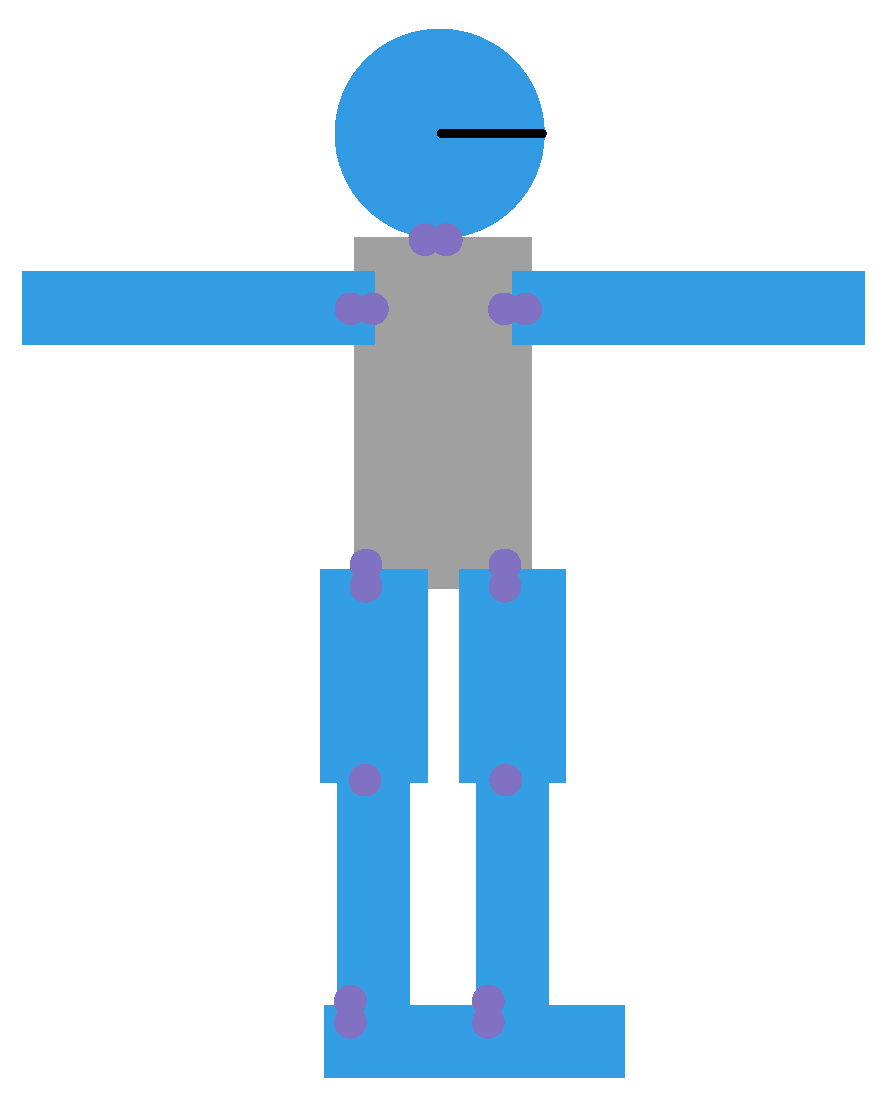
\includegraphics[scale=0.25]{humanoid-2d}
 \caption{Representation of 2D humanoid}
\end{figure}

Environment definition:
\begin{itemize}
 \item \textbf{Observation Space:} The Observation Space is a vector of size 8, containing the angles for each of the 8 joints of the humanoid.
 \begin{table}[H]
 \caption{Observation Space for the 2D Walker environment}
 \centering
 \begin{tabular}{|l|l|l|}
 \hline
 Observation & Min & Max \\ \hline
 Joint Position & -20° & +20° \\ \hline

 \end{tabular}
 \end{table}

 \item \textbf{Action Space:} 
 \begin{table}[H]
 \caption{Action Space for the 2D Walker environment}
 \centering
 \begin{tabular}{|l|l|}
 \hline
 Num & Action \\ \hline
 0 & Move the joint counterclockwise \\ \hline
 1 & Maintain joint position \\ \hline
 2 & Move the joint clockwise \\ \hline
 \end{tabular}
 \end{table}
 \item \textbf{Reward:} 
 \begin{table}[H]
 \caption{Reward system for the 2D Walker environment}
 \centering
 \begin{tabular}{|l|l|}
 \hline
 Action & Points \\ \hline
 Moves Back & 8 \\ \hline
 Stays in Place & 9 \\ \hline
 Moves Forward & 10 \\ \hline
 Loses contact with the ground & cumulative -2 \\ \hline
 Reaches target & 16 \\ \hline
 Falls & 0 \\ \hline
 \end{tabular}
 \end{table}
 
\end{itemize}
The reward is calculated at each timestep, given a threshold $\theta$, the position of the robot is compared to the last position and calculated the offset. If the robot loses contact with the ground with both feet, the reward is subtracted 2 points.
\subsection{3D Walker}
In the 3D environment, the robot needs to simulate the one used by the Bold Hearts team, given that the team already uses a simulator, gazebo, this will be used to interact with the robot given that it provides ROS2 integration.
\begin{figure}[H]
 \centering
 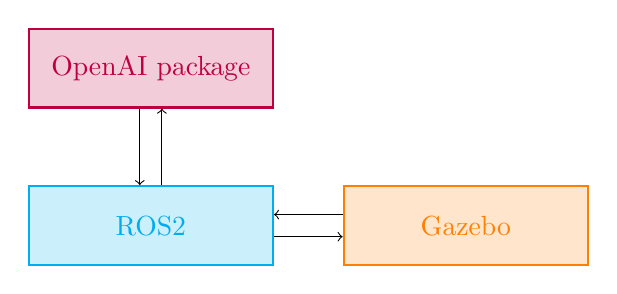
\begin{tikzpicture}[every node/.style=draw]
 \node[rectangle, 
 draw, 
 thick,
 minimum width = 3.1cm,
 minimum height = 1cm,
 color=cyan,
 fill=cyan!20] (A) at (0,0) {ROS2};
 \node[rectangle, 
 draw, 
 thick,
 minimum width = 3.1cm,
 minimum height = 1cm,
 color=purple,
 fill=purple!20] (B) at (0,2) {OpenAI package};
 \node[rectangle, 
 draw, 
 thick,
 minimum width = 3.1cm,
 minimum height = 1cm,
 color=orange,
 fill=orange!20] (C) at (4,0) {Gazebo};

 \draw [->] ([xshift=-4]B.south) to node [midway,left, draw=none]{} ([xshift=-4]A.north);
 \draw [<-] ([xshift=4]B.south) to node [midway,left, draw=none]{} ([xshift=4]A.north);
 \draw [->] ([yshift=-4]A.east) to node [midway,left, draw=none]{} ([yshift=-4]C.west);
 \draw [<-] ([yshift=4]A.east) to node [midway,left, draw=none]{} ([yshift=4]C.west);
 
 \end{tikzpicture}
 \caption{Integration of ROS2, Gazebo and OpenAI Gym}
\end{figure}

To achieve this integration, OpenAI Gym should be able to subscribe ROS2 topics containing the world observations. 
The OpenAI Gym should also be able to publish to ROS2 topics, allowing it to control the robot's joints, as well as call services in order to control the simulation, including pause, unpause and reset the simulation.
One of the main aspects of this integration is to allow to train not only walking but also any relevant task by the team. To achieve this, the OpenAI Gym package should be split into three different files:
\begin{itemize}
 \item Robot
 \item Environment
 \item Task
\end{itemize}
The robot file should contain all the setup required for the Boldbot, the team's robot. On the Environment file, the observation space, action space, reward system and other core Gym functions should be defined. 
Finally, the task file should be specific for the task trying to be achieved, allowing the team to set up just the task without requiring setting up the robot and environment every time.
\cite{ros-gym} 

\begin{figure}[H]
 \centering
 \includegraphics[width=1\linewidth]{boldbot_sim.png}
 \caption{Bold Hearts simulation, the robot, field, goals and ball are simulated }
\end{figure}

The 3D Walker will be using the current simulator, demonstrated above, using the already modelled humanoid and field.

